\documentclass[a4paper,13pt]{article}
\usepackage[T1]{fontenc}
\usepackage[utf8x]{inputenc}
\usepackage[italian,english]{babel}
\usepackage{amssymb,latexsym,amsfonts,amsmath}
\usepackage{lipsum}
\usepackage{url}
\usepackage{graphicx}
\begin{document}
\author{Andrea Pagliaro , Alessio Susco, Shanj Raul Ken Zaccaretti}
\title{Studio e Progettazione del controllo sulla velocità di rotazione di un generatore eolico}
\maketitle
\section{Introduzione}
\section{Modello del sistema}
Per lo studio e la progettazione di un controllore lineare che regoli la rotazione di una turbina eolica in modo che sia costante mediante il pitch , sono state prese in considerazione varie equazioni riguardanti il moto di un rotore e le relative potenze ricavate.
Come le seguenti :
\begin{equation}
P=\frac{1}{2}\,\rho\,A\,C_p\,V_w^3
\end{equation}
Che rappresenta la quantit\'a di potenza assorbita dal rotore della turbina eolica presa in considerazione.
Il Cp \'e il coefficiente di potenza dipendente da $\lambda$ e $\beta$.
Dove a loro volta $\lambda$ \'e dato da :
\begin{equation}
\lambda=\frac{\Omega\,R}{V_w}
\end{equation}
Che viene chiamato tip-speed ratio ed \'e dato dal rapporto tra la velocità angolare
del rotore per il suo raggio e la velocità del vento.
Mentre $\beta$ rappresenta l'angolo di pitch relativo alle pale.
Chiaramente la funzione del coefficiente di potenza comporta delle dinamiche non 
lineari dipendenti dalla geometria del rotore questo a sua volta si ripercuote sull'intero sistema che lo rende non lineare.  
Ora provando a linearizzare il sistema ci \'e risultato molto difficile e solo dopo aver letto alcune pubblicazioni sullo studio di turbine eoliche siamo riusciti a trovare alcune linearizzazioni compiute mediante metodi numerici, che ci hanno permesso di riscrivere il sistema nella seguente forma:
\begin{equation}
\dot{x}=\frac{\gamma}{I_{rot}}x1+\frac{\sigma}{I_{rot}}\,\delta_\beta+\frac{\alpha}{I_{rot}}\,\delta_\omega
\end{equation}
Dove $x$ , lo stato del sistema rappresenta la velocità angolare del rotore ,
$\delta_\beta$ \'e l'ingresso relativo alla perturbazione da parte del pitch,
$\delta_\omega$ \'e la perturbazione relativa alla velocità del vento.
Quindi la nostra matrice di stato \'e data da $A=\frac{\gamma}{I_{rot}}$,
e i coefficienti dei rispettivi ingressi/uscite:
$B=\frac{\sigma}{I_{rot}}$
$\Gamma=\frac{\alpha}{I_{rot}}$
Irot rappresenta inerzia del rotore.
I valori $\gamma$ , $\sigma$ , $\alpha$ rappresentano le derivate parziali ricavate attraverso 
l'equazione dell'aerodinamica del rotore descritta in tal modo:
\begin{equation}
T_{aero}=T(\omega_0,\Omega_0,\beta_0)+\frac{\delta \, T_{aero}}{\delta \, \Omega}+
\frac{\delta \, T_{aero}}{\delta \, \beta}+\frac{\delta \, T_{aero}}{\delta \, \omega}
\end{equation} 
Dove i coefficienti $\gamma=\frac{\delta \, T_{aero}}{\delta \, \Omega}$=-0.1205
$\sigma=\frac{\delta \, T_{aero}}{\delta \, \beta}$=-2.882,
$\alpha=\frac{\delta \, T_{aero}}{\delta \, \omega}$=0.0658
sono gia noti essendo stati ricavati dalla linearizzazione eseguita mediante un metodo numerico non descritto nella pubblicazione di cui si sta facendo uso per il progetto in questione.
I valori degli stati iniziali sono dati da $\omega_0$=18m/s , $\Omega_0$=42RPM e $\beta_0$=12deg.
%----inzio parte controllo nel xaso continuo
\section{Controllo continuo}
Detto questo siamo passati alla progettazione del controllore scegliendo un controllo PI,ovvero proporzionale-intergrativo.
Per rendere i calcoli delle costanti pi\'u semplici \'e stato effettuato un cambio di variabile.
\'E stato quindi posto e come l'errore tra l'uscita e il riferimento
\begin{equation}
e=x-xr        poich\'e y=C*x    dove C=1
\end{equation}
La sua derivata e' rappresentata quindi come :

Lo schema del sistema con relativo controllo e circuito nel caso continuo \'e rappresentato da:
\begin{center}
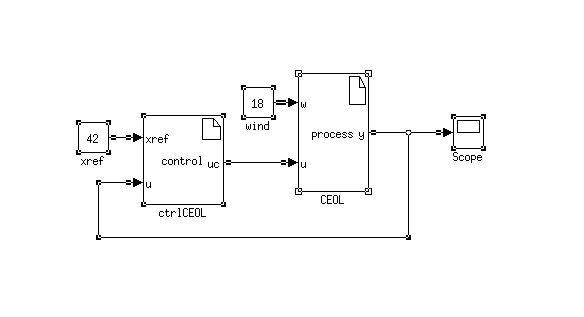
\includegraphics[scale=0.6]{eolcont.png}
\end{center}
\subsection{Grafici sul controllo continuo}
\begin{center}
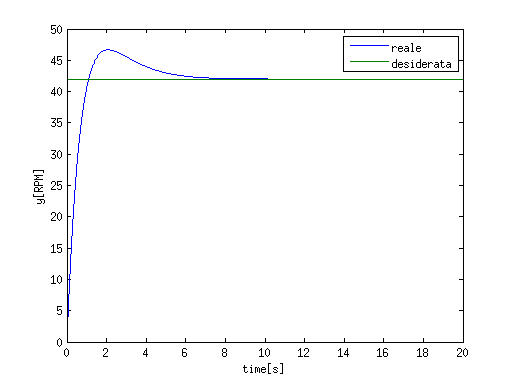
\includegraphics[scale=0.6]{graph/ycont.png}
\end{center}
\begin{center}
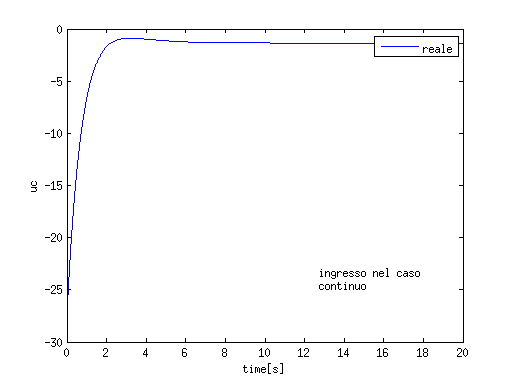
\includegraphics[scale=0.6]{graph/ucont.png}
\end{center}

%-------------Inizio parte discreta-----------------------

\section{Controllo discreto con Event Triggering}

	In questa parte parleremo del controllo discreto con ET della velocità di rotazione di una pala eolica mediante un
	controllore PI.\\ Qui di seguito lo schema di controllo, dove possiamo notare le prime differenze dallo schema 				precedente.
	
\begin{center}
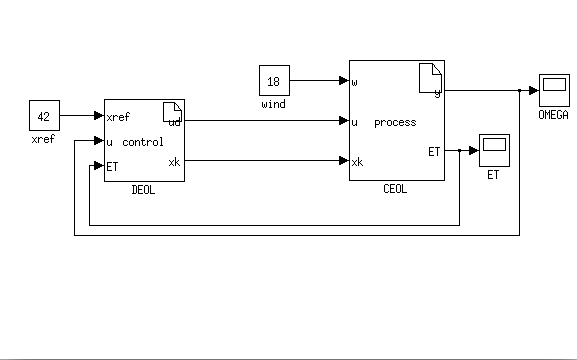
\includegraphics[scale=0.6]{eoltrig.png}
\end{center}

	Rispetto allo schema del controllo continuo osserviamo la presenza di un nuovo ramo diretto, dotato a sua volta di un
	feedback per la gestione dell'ET.\\ \\ \\ \\
	Per iniziare calcoliamo i coefficienti di proporzionalità e di integrazione del controllo PI, partendo dal seguente 		modello di controllo:\\
\begin{equation*}
	u=u_{r}+K_{p}x+K_{i}\int_{0}^{t} x \, d\tau              %------------------modello del controllo---------------
\end{equation*}	
\subsection{Assegnazione degli autovalori}

	Per calcolarli utilizzeremo la formula di Ackermann, ma abbiamo prima bisogno di esplicitare il modello dello spazio 		di
	stato in esame:

%-----Spazio di stato del sistema---
\[Plant	:
\begin{cases}
	
	\dot{I_{e}}= e \\
	\dot{e} = ae + bu
	
\end{cases}\]
%-----------------------------------
	Questo perchè sappiamo che l'errore è dato da:

\begin{equation*}
	e=x-x_{r}          %--------------------errore---------------------------
\end{equation*}
	
	e la dinamica dello stato è:
%-----derivata dello stato-----	
\begin{equation*}
	\dot{x}=ax+bu+\gamma w_{d}    %-----------------derivata dello stato------------ 
\end{equation*} \\
	
	Quindi:

\begin{equation*}
	\dot{e}=\dot{x}=a(e+x_{r})+bu+\gamma w_{d}\,\,\:           %-------------spiegazione equazione--------
	\Rightarrow u=-\frac{\gamma}{b} w_{d}-\frac{a}{b} x_{r}
\end{equation*} \\

	Arrivati a questo punto, dal modello di spazio stato\\
\begin{equation*}	
\begin{pmatrix}
	
	\dot{I_{e}} \\ \dot{e}
	
\end{pmatrix} =         %---------uguale a---------
\begin{pmatrix}

	0&1\\0&a

\end{pmatrix}
\begin{pmatrix}

	I_{e}\\e

\end{pmatrix} +           %------- + ------------
\begin{pmatrix}

	0\\b

\end{pmatrix} u
\end{equation*} \\

	Esplicitiamo la matrice dinamica A:        %-------matrice A------------
\begin{equation*}
\begin{pmatrix}

	0&1\\0&a

\end{pmatrix}
\end{equation*} \\

	e la matrice ingresso-uscita B:          %--------matrice B-------------
\begin{equation*}
\begin{pmatrix}

	0\\b

\end{pmatrix}
\end{equation*} \\


	A questo punto per Ackermann abbiamo bisogno che la matrice di raggiungibilità abbia rango pieno, essendo quest'ultima 	il più grande sottospazio \\A-invariante contenuto nell'immagine di B.\\ \\
	Quindi:
	
\begin{equation*}
	\rho(\mathcal{R}):=
\rho(\:\begin{bmatrix}

	B&AB

\end{bmatrix}\:)=^{?}\rho_{max}=2
\end{equation*}

	Verifichiamo il tutto:
	
\begin{equation*}
\begin{bmatrix}

	B&AB

\end{bmatrix} =              %--------------uguale a-----------------
\begin{bmatrix}

	0&b\\b&ab

\end{bmatrix}
\end{equation*}

	Essendo $b=-2.8818$ abbiamo che il determinante della matrice  2x2 in esame risulta essere diverso da 0,
	e quindi il rango è pieno e pari a 2.\\
	Passiamo ad applicare la formula di Ackermann:
	
\begin{equation*}                    %----------Ackermann Formula------------
	K=
\begin{pmatrix}

	K_{1}&K_{2}

\end{pmatrix} =						%--------------uguale a----------------
\begin{pmatrix}

	K_{i}&K_{p}						

\end{pmatrix} = -					%--------------uguale a meno--------------
\begin{pmatrix}

	0&1						

\end{pmatrix}
\begin{pmatrix}

	B&AB					

\end{pmatrix}^{-1}p(A)
\end{equation*} \\

		Dove p(A) è il polinomio caratteristico p($\lambda$) desiderato con $\lambda=A$.\\\\
	In questo caso per assegnare due autovalori in -1 è stato scelto il seguente polinomio:\\

\begin{equation*}
	p(\lambda)_{des}=(\lambda+1)^{2}=\lambda^{2}+2\lambda+1        %---------------polinomio caratteristico------------
\end{equation*} \\
	
	ottenendo una matrice triangolare superiore
	
\begin{equation*}
	p(A)=A^{2}+2A+I_{2}=
\begin{pmatrix}

	1&a+2\\0&a^{2}+2a+1

\end{pmatrix}
\end{equation*} \\ \\

	La matrice dei coefficienti da trovare può ora essere calcolata come segue:

\begin{equation*}
	K=
\begin{pmatrix}

	K_{1}&K_{2}

\end{pmatrix} =                  %---------uguale a----------------
\begin{pmatrix}

	-\frac{1}{b}&0

\end{pmatrix}
\begin{pmatrix}

	1&a+2\\0&a^{2}+2a+1

\end{pmatrix} =                   %---------uguale a----------------
\begin{pmatrix}

	-\frac{1}{b}&-\frac{a+2}{b}

\end{pmatrix} =                    %---------uguale a----------------
\begin{pmatrix}

	K_{i}&K_{p}

\end{pmatrix} =                    %---------uguale a----------------
\begin{pmatrix}

	0.347&0.652

\end{pmatrix}
\end{equation*}\\
\subsection{Ottimizzazione del criterio d'arresto}
	Un altro problema da affrontare è il calcolo della norma del prodotto PBK.
	Abbiamo bisogno di questo valore per gestire in maniera ottimale la soglia del criterio d'arresto nell'ET.\\
	Per ottenere il prodotto in esame, abbiamo bisogno della matrice P, soluzione dell'equazione di Sylvester, essendo già 	note le matrici B e K.\\ \\ \\ \\
	Ciò vale, tenendo conto della matrice dinamica $A_{c}$ :\\
	
\begin{equation*}
	A_{c}=A+BK=
\begin{pmatrix}

	0&1\\-0.0418&-2.9604

\end{pmatrix}
\end{equation*} \\
	
	Per risolvere l'equazione di Sylvester
	
\begin{equation*}
	A_{c}^{T}P + PA_{c} = -Q              %------------equazione di Sylvester----------------
\end{equation*}

	Scegliamo una matrice Q definita postiva, a piacere.\\
	Per le nostre simulazioni abbiamo utilizzato una matrice Q del tipo:\\

\begin{equation*}
	Q=
\begin{pmatrix}

	\frac{1}{2}&0\\0&657

\end{pmatrix}
\end{equation*}\\
	
	Ottenendo la matrice P dall'equazione di Sylvester mediante il MATLAB:\\
	
\begin{equation*}
	P=
\begin{pmatrix}

	22.4210&5.9774\\5.9774&112.9844

\end{pmatrix}
\end{equation*}\\

	E' possibile quindi calcolare il prodotto PBK ed applicarne la norma 2:\\
	
\begin{equation*}
	PBK=
\begin{pmatrix}

	-0.2500&-0.4697\\-4.7255&-8.8789

\end{pmatrix}
	\Rightarrow norm_{2}(PBK)=10.0722
\end{equation*}\\

	L'indice relativo al trigger, $\rho_{max}$ sarà dato infine da:
	
\begin{equation*}
	\rho_{max}=2\frac{\theta}{20.1443} \lambda_{min}^{Q}
\end{equation*}\\

	con $\lambda_{min}^{Q}$ autovalore minimo della matrice Q, ovvero pari a 0.5 .\\
	
	Il $\rho_{max}$ viene utilizzato come indice di peso per la commutazione del coefficiente dell'ET nel codice sorgente.
	\\ Il coefficiente dell'ET assumerà valore pari a 0, ovvero non agendo sul controllore, se il modulo dell'errore        	$n_{e}$ si mantiene sotto una certa soglia, definita proprio da:
	
\begin{equation*}
	n_{r}=\rho_{max}n_{x}
\end{equation*}

	con $n_{x}$ modulo dell'uscita.
	Altrimenti l'ET assume valore pari a 1, agendo sul sistema e quindi andando a stabilizzare il controllo.
	
\subsection{Grafici sul controllo discreto}

\begin{center}
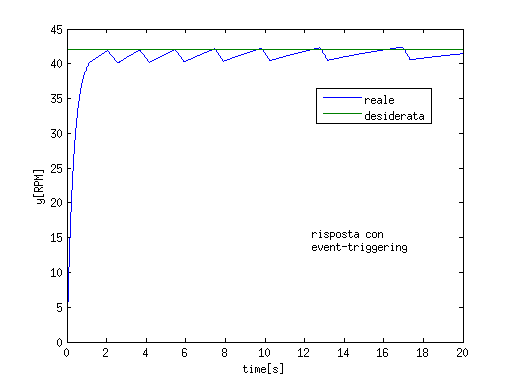
\includegraphics[scale=0.6]{graph/ydisc.png}
\end{center}
\begin{center}
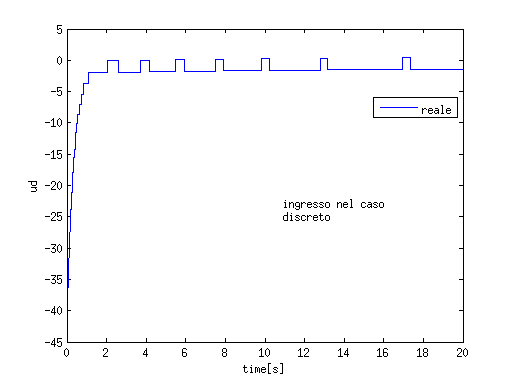
\includegraphics[scale=0.6]{graph/udisc.png}
\end{center}



\end{document}


